%%%%%%%%%%%%%%%%%%%%%%%%%%%%%%%%%%%%%%%%%
% Beamer Presentation
% LaTeX Template
% Version 1.0 (10/11/12)
%
% This template has been downloaded from:
% http://www.LaTeXTemplates.com
%
% License:
% CC BY-NC-SA 3.0 (http://creativecommons.org/licenses/by-nc-sa/3.0/)
%
%%%%%%%%%%%%%%%%%%%%%%%%%%%%%%%%%%%%%%%%%

%----------------------------------------------------------------------------------------
%	PACKAGES AND THEMES
%----------------------------------------------------------------------------------------

\documentclass{beamer}

\mode<presentation> {
	
	% The Beamer class comes with a number of default slide themes
	% which change the colors and layouts of slides. Below this is a list
	% of all the themes, uncomment each in turn to see what they look like.
	
	%\usetheme{default}
	%\usetheme{AnnArbor}
	%\usetheme{Antibes}
	%\usetheme{Bergen}
	%\usetheme{Berkeley}
	%\usetheme{Berlin}
	%\usetheme{Boadilla}
	%\usetheme{CambridgeUS}
	%\usetheme{Copenhagen}
	%\usetheme{Darmstadt}
	%\usetheme{Dresden}
	%\usetheme{Frankfurt}
	%\usetheme{Goettingen}
	%\usetheme{Hannover}
	%\usetheme{Ilmenau}
	%\usetheme{JuanLesPins}
	%\usetheme{Luebeck}
	\usetheme{Madrid}
	%\usetheme{Malmoe}
	%\usetheme{Marburg}
	%\usetheme{Montpellier}
	%\usetheme{PaloAlto}
	%\usetheme{Pittsburgh}
	%\usetheme{Rochester}
	%\usetheme{Singapore}
	%\usetheme{Szeged}
	%\usetheme{Warsaw}
	
	% As well as themes, the Beamer class has a number of color themes
	% for any slide theme. Uncomment each of these in turn to see how it
	% changes the colors of your current slide theme.
	
	%\usecolortheme{albatross}
	%\usecolortheme{beaver}
	%\usecolortheme{beetle}
	%\usecolortheme{crane}
	%\usecolortheme{dolphin}
	%\usecolortheme{dove}
	%\usecolortheme{fly}
	%\usecolortheme{lily}
	%\usecolortheme{orchid}
	%\usecolortheme{rose}
	%\usecolortheme{seagull}
	%\usecolortheme{seahorse}
	%\usecolortheme{whale}
	%\usecolortheme{wolverine}
	
	%\setbeamertemplate{footline} % To remove the footer line in all slides uncomment this line
	%\setbeamertemplate{footline}[page number] % To replace the footer line in all slides with a simple slide count uncomment this line
	
	%\setbeamertemplate{navigation symbols}{} % To remove the navigation symbols from the bottom of all slides uncomment this line
}

\usepackage{graphicx} % Allows including images
\usepackage{booktabs} % Allows the use of \toprule, \midrule and \bottomrule in tables

\usepackage{xcolor}
\usepackage{xspace}
\usepackage{algorithm}
\usepackage{algorithmic}
\usepackage{caption}
\usepackage{multirow}
\usepackage{fancyvrb}

\usepackage{tikz}
\usetikzlibrary{matrix, decorations, patterns, positioning, shapes, calc, intersections, arrows, fit}
\newcommand\addvmargin[1]{
	\node[fit=(current bounding box),inner ysep=#1,inner xsep=0]{};
}



\newcommand{\tensor}[1]{{\cal\textbf{#1}\xspace}}
\newcommand{\ttrain}{{\it Tensor-Train}\xspace}


%% Colors from https://latexcolor.com/
\definecolor{pastelviolet}{rgb}{0.8, 0.6, 0.79}
\definecolor{babyblueeyes}{rgb}{0.63, 0.79, 0.95}
\definecolor{pastelyellow}{rgb}{0.99, 0.99, 0.59}
\definecolor{pastelgreen}{rgb}{0.47, 0.87, 0.47}
\definecolor{pastelred}{rgb}{1.0, 0.41, 0.38}
\colorlet{patternblue}{blue!60}


%%Fast algorithms for matrix multiplication and tensor operations
%%Traditional matrix multiplication performs O(n^3) operations to multiply two square matrices of dimension n. Strassen Surprised the world in 1969 with an algorithm which performs less arithmetic operations than the traditional one. His work is based on the representation of a 2X2 matrix multiplication as a canonical tensor decomposition of a 4X4X4 tensor. First, I will talk about state-of-the-art approaches to perform traditional matrix multiplication on modern computing systems and then talk about extending the concept of Strassen to perform tensor contraction operations.
%%
%%This talk is based on a joint work with Laura Grigori (Inria Paris, France), and Grey Ballard (Wake Forest University, USA).

%----------------------------------------------------------------------------------------
%	TITLE PAGE
%----------------------------------------------------------------------------------------

\title[Fast Algorithms for Tensors]{Fast Algorithms for Matrix Multiplication and Tensor Operations} % The short title appears at the bottom of every slide, the full title is only on the title page

\author{Suraj Kumar} % Your name
\institute[Inria Paris] % Your institution as it will appear on the bottom of every slide, may be shorthand to save space
{
	Alpines team, Inria Paris, France\\ % Your institution for the title page
	\medskip
	\textit{Suraj.kumar@inria.fr} % Your email address
}

%%Séminaire d’Analyse Numérique et Calcul Scientifique
\date{March 4, 2021} % Date, can be changed to a custom date

\begin{document}
	
\begin{frame}
	\titlepage % Print the title page as the first slide
\end{frame}


%%\section{Introduction}
\begin{frame}{Collaborators}
This is joint work with ...
\begin{itemize}
	\item Laura Grigori -- Inria Paris, France
	\item Grey Ballard -- Wake Forest University, USA
	\item Hussam Al Daas -- STFC Rutherford Appleton Laboratory, UK
	\item Olivier Beaumont -- Inria Bordeaux, France
\end{itemize}
\end{frame}
\section{Traditional Matrix Multiplication}

\begin{frame}
\frametitle{Overview} % Table of contents slide, comment this block out to remove it
\tableofcontents % Throughout your presentation, if you choose to use \section{} and \subsection{} commands, these will automatically be printed on this slide as an overview of your presentation
\end{frame}

%------------------------------------------------
\begin{frame}
\frametitle{Table of Contents}
\tableofcontents[currentsection]
\end{frame}
%----------------------------------------------------------------------------------------
%	PRESENTATION SLIDES
%----------------------------------------------------------------------------------------


\begin{frame}{Traditional matrix multiplication}
\begin{itemize}
	\item $C= AB$, where $A \in\mathbb{R}^{m \times k}$, $B \in\mathbb{R}^{k \times n}$, and  $C$ $\in$ $\mathbb{R}^{m \times n}$.
	\item $C_{ij} = \sum_p A_{ip}*B_{pj}$
\end{itemize}
For simplicity, we assume $m=k=n$ throughout the presentation.
\begin{center}
	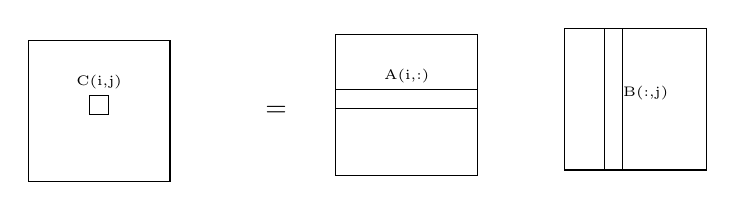
\begin{tikzpicture}[scale=1, every node/.style={transform shape}]
%%	\tikzstyle{taskr}=[draw=black, minimum height=18mm, minimum width=18mm, anchor=south west, fill=pastelgreen, text=black]

	\tikzstyle{taskr}=[draw=black, minimum height=18mm, minimum width=18mm, fill=pastelgreen, text=black]
	
	\tikzstyle{taskrow}=[draw=black, minimum height=2mm, minimum width=18mm, fill=pastelgreen, fill=none, text=black]
	\tikzstyle{taskcol}=[draw=black, minimum height=18mm, minimum width=2mm, fill=pastelgreen, fill=none, text=black]
	
	\tikzstyle{taskrsmall}=[draw=black, minimum height=2mm, minimum width=2mm, fill=none, text=black]

%%	\node(t1) at (0,0) {};
%%	\node [above right=0cm and 0cm of t1.mid,taskr](T1) {};
	\node [taskr, fill=none] (T1) at (0,0) {};
	\node [taskrsmall] (T2) at (T1.mid) {};
	\node [above] at (T2.mid) {\tiny C(i,j)};
	\node[draw=none, text=black, scale=1] at (2.25,0) {$=$};
	
	\node [right=3cm of T1.mid,taskr, fill=none](T3) {};
	\node[taskrow](T4) at (T3.mid) {};
	\node [above] at (T4.mid) {\tiny A(i,:)};
	
	\node [right=2cm of T3.mid,taskr, fill=none](T5) {};
	\node [right=2.5cm of T3.mid, taskcol](T6) {};
	\node [right] at (T6.mid) {\tiny B(:,j)};
	
	\end{tikzpicture}
\end{center}
\end{frame}


\begin{frame}{Matrix multiplication: linear combination of columns}
\begin{itemize}
	\item A column of $C$ is obtained by linear combination of columns of $A$.
\end{itemize}
\begin{center}
	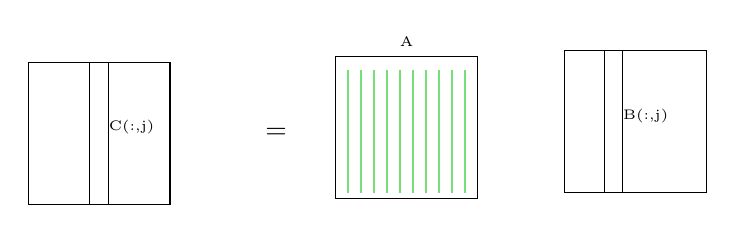
\begin{tikzpicture}[scale=1, every node/.style={transform shape}]
	%%	\tikzstyle{taskr}=[draw=black, minimum height=18mm, minimum width=18mm, anchor=south west, fill=pastelgreen, text=black]
	
	\tikzstyle{taskr}=[draw=black, minimum height=18mm, minimum width=18mm, fill=pastelgreen, text=black]
	
	\tikzstyle{taskrow}=[draw=black, minimum height=2mm, minimum width=18mm, fill=pastelgreen, fill=none, text=black]
	\tikzstyle{taskcol}=[draw=black, minimum height=18mm, minimum width=2mm, fill=pastelgreen, fill=none, text=black]
	
	\tikzstyle{taskrsmall}=[draw=black, minimum height=2mm, minimum width=2mm, fill=none, text=black]
	
	%%	\node(t1) at (0,0) {};
	%%	\node [above right=0cm and 0cm of t1.mid,taskr](T1) {};
	\node [taskr, fill=none] (T1) at (0,0) {};
	\node [taskcol] (T2) at (0,0) {};
	\node [right] at (T2.mid) {\tiny C(:,j)};
	
	\node[draw=none, text=black, scale=1] at (2.25,0) {$=$};
%%	
	\node [right=3cm of T1.mid,taskr, fill=none](T3) {};
%%	\node[taskrow](T4) at (T3.mid) {};
	\node [above] at (T3.north) {\tiny A};
%%	\draw[pastelgreen, thick] (3.1cm, 0.8) -- (3.1cm, -0.75);
%%	\draw[pastelgreen, thick] (3.2cm, 0.8) -- (3.2cm, -0.75);
%%	\draw[pastelgreen, thick] (3.3cm, 0.8) -- (3.3cm, -0.75);
%%	\draw[pastelgreen, thick] (3.45cm, 0.8) -- (3.45cm, -0.75);
   \foreach \x in {1,2,3,4,5,6,7,8,9,10}
    \draw [pastelgreen, thick] (3+0.165* \x, 0.8) -- (3+0.165* \x, -0.75);
%%  \foreach \y [count=\yi] in {0,...,3}  
%%  \draw (\x\y)--(\x\yi) (\y\x)--(\yi\x) ;

%%	
	\node [right=2cm of T3.mid,taskr, fill=none](T5) {};
	\node [right=2.5cm of T3.mid, taskcol](T6) {};
	\node [right] at (T6.mid) {\tiny B(:,j)};
%%	
	\end{tikzpicture}
\end{center}
\end{frame}

\begin{frame}{Matrix multiplication: linear combination of rows}
\begin{itemize}
	\item A row of $C$ is obtained by linear combination of rows of $B$.
\end{itemize}
\begin{center}
	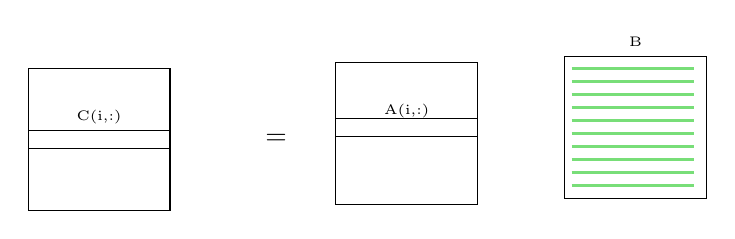
\begin{tikzpicture}[scale=1, every node/.style={transform shape}]
	%%	\tikzstyle{taskr}=[draw=black, minimum height=18mm, minimum width=18mm, anchor=south west, fill=pastelgreen, text=black]
	
	\tikzstyle{taskr}=[draw=black, minimum height=18mm, minimum width=18mm, fill=pastelgreen, text=black]
	
	\tikzstyle{taskrow}=[draw=black, minimum height=2mm, minimum width=18mm, fill=pastelgreen, fill=none, text=black]
	\tikzstyle{taskcol}=[draw=black, minimum height=18mm, minimum width=2mm, fill=pastelgreen, fill=none, text=black]
	
	\tikzstyle{taskrsmall}=[draw=black, minimum height=2mm, minimum width=2mm, fill=none, text=black]
	
	%%	\node(t1) at (0,0) {};
	%%	\node [above right=0cm and 0cm of t1.mid,taskr](T1) {};
	\node [taskr, fill=none] (T1) at (0,0) {};
	\node [taskrow] (T2) at (0,0) {};
	\node [above] at (T2.mid) {\tiny C(i,:)};
	
	\node[draw=none, text=black, scale=1] at (2.25,0) {$=$};
	%%	
	\node [right=3cm of T1.mid,taskr, fill=none](T3) {};
	\node[taskrow](T4) at (T3.mid) {};
	\node [above] at (T3.mid) {\tiny A(i,:)};
%%	\node [above] at (T3.north) {\tiny A};
	%%	\draw[pastelgreen, thick] (3.1cm, 0.8) -- (3.1cm, -0.75);
	%%	\draw[pastelgreen, thick] (3.2cm, 0.8) -- (3.2cm, -0.75);
	%%	\draw[pastelgreen, thick] (3.3cm, 0.8) -- (3.3cm, -0.75);
	%%	\draw[pastelgreen, thick] (3.45cm, 0.8) -- (3.45cm, -0.75);
%%	\foreach \x in {1,2,3,4,5,6,7,8,9,10}
%%		\draw [pastelgreen, thick] (3+0.165* \x, 0.8) -- (3+0.165* \x, -0.75);
	%%  \foreach \y [count=\yi] in {0,...,3}  
	%%  \draw (\x\y)--(\x\yi) (\y\x)--(\yi\x) ;
	
	%%	
	\node [right=2cm of T3.mid,taskr, fill=none](T5) {};
	\node [above] at (T5.north) {\tiny B};

	\foreach \x in {1,2,3,4,5,6,7,8,9,10}
		\draw [pastelgreen, thick] (6, -0.75+0.165* \x) -- (7.56, -0.75+0.165* \x);
	
%%	\node [right=2.5cm of T3.mid, taskcol](T6) {};
%%	\node [right] at (T6.mid) {\tiny B(:,j)};
	%%	
	\end{tikzpicture}
\end{center}

\end{frame}

\begin{frame}{Matrix multiplication: sum of $n$ matrices}
\begin{itemize}
	\item Matrix multiplication can also be viewed as sum of $n$ matrices.
\end{itemize}
\begin{center}
	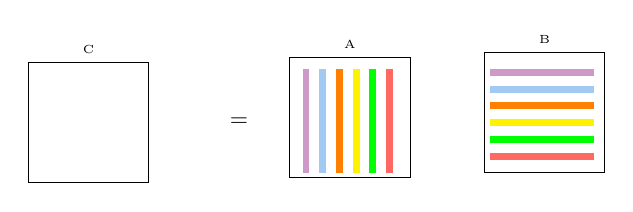
\begin{tikzpicture}[scale=0.85, every node/.style={transform shape}]
	%%	\tikzstyle{taskr}=[draw=black, minimum height=18mm, minimum width=18mm, anchor=south west, fill=pastelgreen, text=black]
	
	\tikzstyle{taskr}=[draw=black, minimum height=18mm, minimum width=18mm, fill=pastelgreen, text=black]
	
	\tikzstyle{taskrow}=[draw=black, minimum height=2mm, minimum width=18mm, fill=pastelgreen, fill=none, text=black]
	\tikzstyle{taskcol}=[draw=black, minimum height=18mm, minimum width=2mm, fill=pastelgreen, fill=none, text=black]
	
	\tikzstyle{taskrsmall}=[draw=black, minimum height=2mm, minimum width=2mm, fill=none, text=black]
	
	%%	\node(t1) at (0,0) {};
	%%	\node [above right=0cm and 0cm of t1.mid,taskr](T1) {};
	\node [taskr, fill=none] (T1) at (0,0) {};
%%	\node [taskrow] (T2) at (0,0) {};
	\node [above] at (T1.north) {\tiny C};
	
	\node[draw=none, text=black, scale=1] at (2.25,0) {$=$};
	%%	
	\node [right=3cm of T1.mid,taskr, fill=none](T3) {};
%%	\node[taskrow](T4) at (T3.mid) {};
%%	\node [above] at (T3.mid) {\tiny A(i,:)};
		\node [above] at (T3.north) {\tiny A};
	%%	\draw[pastelgreen, thick] (3.1cm, 0.8) -- (3.1cm, -0.75);
	%%	\draw[pastelgreen, thick] (3.2cm, 0.8) -- (3.2cm, -0.75);
	%%	\draw[pastelgreen, thick] (3.3cm, 0.8) -- (3.3cm, -0.75);
	%%	\draw[pastelgreen, thick] (3.45cm, 0.8) -- (3.45cm, -0.75);´
%%	  \foreach \x/\xtext in {0,...,3,2.72 / e} 
	\foreach \x/\y in {1/pastelviolet, 2/babyblueeyes, 3/orange, 4/yellow, 5/green, 6/pastelred}
		\draw [\y, line width = 2.5] (3+0.25* \x, 0.8) -- (3+0.25* \x, -0.75);
	%%  \foreach \y [count=\yi] in {0,...,3}  
	%%  \draw (\x\y)--(\x\yi) (\y\x)--(\yi\x) ;
	
	%%	
	\node [right=2cm of T3.mid,taskr, fill=none](T5) {};
	\node [above] at (T5.north) {\tiny B};
	
	\foreach \x/\y in {1/pastelviolet, 2/babyblueeyes, 3/orange, 4/yellow, 5/green, 6/pastelred}
	\draw [\y, line width = 2.5] (6, 1-0.25* \x) -- (7.56, 1-0.25* \x);
	
	%%	\node [right=2.5cm of T3.mid, taskcol](T6) {};
	%%	\node [right] at (T6.mid) {\tiny B(:,j)};
	%%	
	\end{tikzpicture}
\end{center}

\begin{center}
	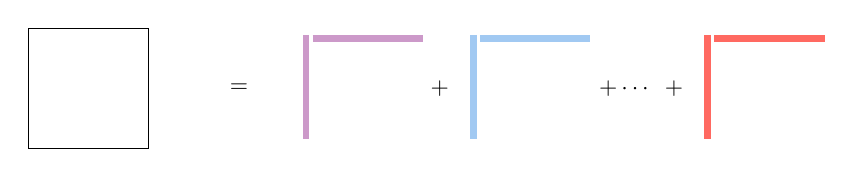
\begin{tikzpicture}[scale=0.85, every node/.style={transform shape}]
	%%	\tikzstyle{taskr}=[draw=black, minimum height=18mm, minimum width=18mm, anchor=south west, fill=pastelgreen, text=black]
	
	\tikzstyle{taskr}=[draw=black, minimum height=18mm, minimum width=18mm, fill=pastelgreen, text=black]
	
	
	%%	\node(t1) at (0,0) {};
	%%	\node [above right=0cm and 0cm of t1.mid,taskr](T1) {};
	\node [taskr, fill=none] (T1) at (0,0) {};
	%%	\node [taskrow] (T2) at (0,0) {};
%%	\node [above] at (T1.north) {\tiny C};
	
	\node[draw=none, text=black] at (2.25,0) {$=$};
	
	\draw [pastelviolet, line width = 2.5] (3+0.25, 0.8) -- (3+0.25, -0.75);
	\draw [pastelviolet, line width = 2.5] (3+0.35, 1-0.25) -- (5, 1-0.25);
	\node[draw=none, text=black] at (5.25,0) {$+$};
	
	\draw [babyblueeyes, line width = 2.5] (2.5+3+0.25, 0.8) -- (2.5+3+0.25, -0.75);
	\draw [babyblueeyes, line width = 2.5] (2.5+3+0.35, 1-0.25) -- (2.5+5, 1-0.25);
	\node[draw=none, text=black] at (2.75+5.25,0) {$+\cdots$};
	
	\node[draw=none, text=black] at (3.5+5.25,0) {$+$};
	\draw [pastelred, line width = 2.5] (9.25, 0.8) -- (9.25, -0.75);
	\draw [pastelred, line width = 2.5] (9.35, 1-0.25) -- (9.35+1.65, 1-0.25);
	
	%%	
%%	\node [right=3cm of T1.mid,taskr, fill=none](T3) {};
%%	%%	\node[taskrow](T4) at (T3.mid) {};
%%	%%	\node [above] at (T3.mid) {\tiny A(i,:)};
%%	\node [above] at (T3.north) {\tiny A};
%%	%%	\draw[pastelgreen, thick] (3.1cm, 0.8) -- (3.1cm, -0.75);
%%	%%	\draw[pastelgreen, thick] (3.2cm, 0.8) -- (3.2cm, -0.75);
%%	%%	\draw[pastelgreen, thick] (3.3cm, 0.8) -- (3.3cm, -0.75);
%%	%%	\draw[pastelgreen, thick] (3.45cm, 0.8) -- (3.45cm, -0.75);´
%%	%%	  \foreach \x/\xtext in {0,...,3,2.72 / e} 
%%	\foreach \x/\y in {1/pastelviolet, 2/babyblueeyes, 3/orange, 4/yellow, 5/green, 6/pastelred}
%%	\draw [\y, line width = 2.5] (3+0.25* \x, 0.8) -- (3+0.25* \x, -0.75);
%%	%%  \foreach \y [count=\yi] in {0,...,3}  
%%	%%  \draw (\x\y)--(\x\yi) (\y\x)--(\yi\x) ;
%%	
%%	%%	
%%	\node [right=2cm of T3.mid,taskr, fill=none](T5) {};
%%	\node [above] at (T5.north) {\tiny B};
%%	
%%	\foreach \x/\y in {1/pastelviolet, 2/babyblueeyes, 3/orange, 4/yellow, 5/green, 6/pastelred}
%%	\draw [\y, line width = 2.5] (6, 1-0.25* \x) -- (7.56, 1-0.25* \x);
%%	
%%	%%	\node [right=2.5cm of T3.mid, taskcol](T6) {};
%%	%%	\node [right] at (T6.mid) {\tiny B(:,j)};
%%	%%	
	\end{tikzpicture}
\end{center}


\end{frame}


\begin{frame}{Matrix multiplication: recursive calls on submatrices}
\begin{itemize}
	\item Matrix is divided into 2$\times$2 blocks
\end{itemize}
%%\begin{pmatrix}
%%	1 & 2 & 3\\
%%	a & b & c
%%\end{pmatrix}

\begin{align*}
\begin{pmatrix}
	C_{11} & C_{12} \\
	C_{21} & C_{22}
\end{pmatrix}
&
=
\begin{pmatrix}
A_{11} & A_{12} \\
A_{21} & A_{22}
\end{pmatrix}
\begin{pmatrix}
B_{11} & B_{12} \\
B_{21} & B_{22}
\end{pmatrix}
\end{align*}

\begin{align*}
C_{11} &= A_{11}B_{11} + A_{12}B_{21}\\
C_{12} &= A_{11}B_{12} + A_{12}B_{22}\\
C_{21} &= A_{21}B_{11} + A_{22}B_{21}\\
C_{22} &= A_{21}B_{12} + A_{22}B_{22}\\
\end{align*}
\end{frame}


\begin{frame}{Matrix multiplication: recursive calls on submatrices}
Operation count recurrence,
\begin{align*}
T(n) &= 8T\Big(\frac{n}{2}\Big) + \mathcal{O}(n^2)\\
T(n) &= 1
\end{align*}
Here $\mathcal{O}(n^2)$ refers that $\exists c\in\mathbb{N}$ such that this term is less than or equal to $cn^2$ for every $n$.
\medskip


After solving, we obtain $T(n) = \mathcal{O}(n^3)$.
\end{frame}


\section{Strassen's Matrix Multiplication}
\begin{frame}
\frametitle{Table of Contents}
\tableofcontents[currentsection]
\end{frame}

\begin{frame}{Matrix multiplication: Strassen's algorithm}
\begin{align*}
\begin{pmatrix}
	C_{11} & C_{12} \\
	C_{21} & C_{22}
\end{pmatrix}
&
=
\begin{pmatrix}
	A_{11} & A_{12} \\
	A_{21} & A_{22}
\end{pmatrix}
\begin{pmatrix}
	B_{11} & B_{12} \\
	B_{21} & B_{22}
\end{pmatrix}
\end{align*}

\begin{minipage}{0.45\columnwidth}
\begin{align*}\small
M_1 &= (A_{11} + A_{22})(B_{11}+B_{22})\\
M_2 &= (A_{21} + A_{22})B_{11}\\
M_3 &= A_{11} (B_{12}-B_{22})\\
M_4 &= A_{22} (B_{21}-B_{11})\\
M_5 &= (A_{11} +A_{12})B_{22}\\
M_6 &= (A_{21}-A_{11})(B_{11} +B_{12})\\
M_7 &= (A_{12}-A_{22})(B_{21} + B_{22}) 
\end{align*}
\end{minipage}
\hfill
\begin{minipage}{0.45\columnwidth}
\begin{center}
	\begin{align*}
	C_{11} &= M_1 + M_4 -M_5 +M_7\\
	C_{12} &= M_3 + M_5\\
	C_{21} &= M_2 + M_4\\
	C_{22} &= M_1 -M_2 + M_3 + M_6
	\end{align*}
\end{center}
\end{minipage}

\end{frame}



\begin{frame}{Matrix multiplication: Strassen's algorithm}
Operation count recurrence,
\begin{align*}
T(n) &= 7T\big(\frac{n}{2}\big) + \mathcal{O}(n^2)\\
T(n) &= 1
\end{align*}
After solving, we obtain $T(n) = \mathcal{O}(n^{\log_2 7})$.\\
$\qquad\qquad\qquad\qquad\qquad\log_2 7 \approx 2.81$
%% \mathcal{O}(n^{2.81})$.
\begin{block}{Questions}
\begin{itemize}
	\item Is there a way to perform matrix multiplication in less number of operations than this algorithm?
	\item What is the minimum number of operations to perform matrix multiplication?
\end{itemize}
\end{block}
\end{frame}

\section{Tensors \& their Low Rank Tensor Representations} % Sections can be created in order to organize your presentation into discrete blocks, all sections and subsections are automatically printed in the table of contents as an overview of the talk
\begin{frame}
\frametitle{Table of Contents}
\tableofcontents[currentsection]
\end{frame}

\begin{frame}{Tensors: multidimensional arrays}
\begin{tabular}{ccc}
	Dimension & Name &\\
	%%\begin{tikzpicture}[scale=0.625, every node/.style={transform shape}]
	%%\tikzstyle{taskr}=[draw=black, minimum height=1mm, minimum width=12mm, anchor=south west, fill=pastelgreen, text=black]
	%%			\node (t01) at (0,0) [taskr]{};
	%%\end{tikzpicture}
	%%\begin{tikzpicture}
	%%\pgfmathsetmacro{\cubex}{5}
	%%\pgfmathsetmacro{\cubey}{1}
	%%\pgfmathsetmacro{\cubez}{3}
	%%\draw[red,fill=yellow] (0,0,0) -- ++(-\cubex,0,0) -- ++(0,-\cubey,0) -- ++(\cubex,0,0) -- cycle;
	%%\draw[red,fill=yellow] (0,0,0) -- ++(0,0,-\cubez) -- ++(0,-\cubey,0) -- ++(0,0,\cubez) -- cycle;
	%%\draw[red,fill=yellow] (0,0,0) -- ++(-\cubex,0,0) -- ++(0,0,-\cubez) -- ++(\cubex,0,0) -- cycle;
	%%\end{tikzpicture}
	%%$0$ & Scalar & \\
	$1$ & Vector & 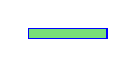
\begin{tikzpicture}[scale=0.25, every node/.style={transform shape}]
	\pgfmathsetmacro{\rectx}{4}
	\pgfmathsetmacro{\recty}{0.5}
	\draw[blue,fill=pastelgreen] (0,0) -- ++(-\rectx,0) -- ++(0,\recty) -- ++(\rectx, 0) -- cycle;
	\end{tikzpicture} \\
	&&\\
	$2$ & Matrix & 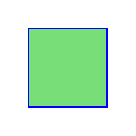
\begin{tikzpicture}[scale=0.25, every node/.style={transform shape}]
	\pgfmathsetmacro{\rectx}{4}
	\pgfmathsetmacro{\recty}{4}
	\draw[blue,fill=pastelgreen] (0,0) -- ++(-\rectx,0) -- ++(0,\recty) -- ++(\rectx, 0) -- cycle;
	%%\addvmargin{4};
	\end{tikzpicture}\\
	&&\\
	$3$ & $3$-dimensional tensor & 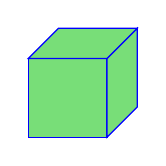
\begin{tikzpicture}[scale=0.25, every node/.style={transform shape}]
	\pgfmathsetmacro{\cubex}{4}
	\pgfmathsetmacro{\cubey}{4}
	\pgfmathsetmacro{\cubez}{4}
	\draw[blue,fill=pastelgreen] (0,0,0) -- ++(-\cubex,0,0) -- ++(0,-\cubey,0) -- ++(\cubex,0,0) -- cycle;
	\draw[blue,fill=pastelgreen] (0,0,0) -- ++(0,0,-\cubez) -- ++(0,-\cubey,0) -- ++(0,0,\cubez) -- cycle;
	\draw[blue,fill=pastelgreen] (0,0,0) -- ++(-\cubex,0,0) -- ++(0,0,-\cubez) -- ++(\cubex,0,0) -- cycle;
	\end{tikzpicture}\\
	&&\\
	$4$ & $4$-dimensional tensor & 
	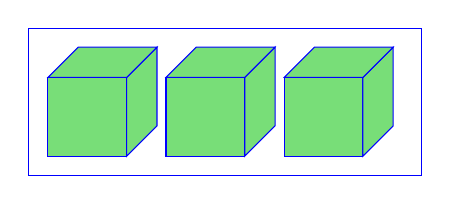
\begin{tikzpicture}[scale=0.25, every node/.style={transform shape}]
	\pgfmathsetmacro{\cubex}{4}
	\pgfmathsetmacro{\cubey}{4}
	\pgfmathsetmacro{\cubez}{4}
	\draw[blue,fill=pastelgreen] (0,0,0) -- ++(-\cubex,0,0) -- ++(0,-\cubey,0) -- ++(\cubex,0,0) -- cycle;
	\draw[blue,fill=pastelgreen] (0,0,0) -- ++(0,0,-\cubez) -- ++(0,-\cubey,0) -- ++(0,0,\cubez) -- cycle;
	\draw[blue,fill=pastelgreen] (0,0,0) -- ++(-\cubex,0,0) -- ++(0,0,-\cubez) -- ++(\cubex,0,0) -- cycle;
	
	\draw[blue,fill=pastelgreen] (\cubex +2,0,0) -- ++(-\cubex,0,0) -- ++(0,-\cubey,0) -- ++(\cubex,0,0) -- cycle;
	\draw[blue,fill=pastelgreen] (\cubex +2,0,0) -- ++(0,0,-\cubez) -- ++(0,-\cubey,0) -- ++(0,0,\cubez) -- cycle;
	\draw[blue,fill=pastelgreen] (\cubex +2,0,0) -- ++(-\cubex,0,0) -- ++(0,0,-\cubez) -- ++(\cubex,0,0) -- cycle;
	
	\draw[blue,fill=pastelgreen] (\cubex +2 + \cubex +2,0,0) -- ++(-\cubex,0,0) -- ++(0,-\cubey,0) -- ++(\cubex,0,0) -- cycle;
	\draw[blue,fill=pastelgreen] (\cubex +2 + \cubex +2,0,0) -- ++(0,0,-\cubez) -- ++(0,-\cubey,0) -- ++(0,0,\cubez) -- cycle;
	\draw[blue,fill=pastelgreen] (\cubex +2 + \cubex +2,0,0) -- ++(-\cubex,0,0) -- ++(0,0,-\cubez) -- ++(\cubex,0,0) -- cycle;
	
	\draw[blue, fill=none] (-\cubex -1, 2.5, 0) -- ++(0, -\cubey -3.5, 0) -- ++(\cubex +2 + \cubex +2 + \cubex + \cubex,0,0) -- ++(0, \cubey +3.5, 0) -- cycle; 
	\end{tikzpicture}
\end{tabular}

\end{frame}

\begin{frame}{Tensors}
\begin{itemize}
	\item Tensors are used in several domains
	\begin{itemize}
		\item Quantum molecular dynamics, signal processing, data mining, neurosciences, computer vision, psychometrics, chemometrics, ...
	\end{itemize}
	\vfill
	\item Memory and computation requirements are exponential in the number of dimensions
	\begin{itemize}
		\item A molecular simulation involving just $100$ spatial orbitals  manipulate a huge tensor with $4^{100}$ elements
		\item People work with low dimensional structure of the tensors
	\end{itemize}
%%	\vfill
%%	\item Limited work on parallelization of tensor algorithms
	%%    \begin{itemize}
	%%    	\item Matricized Tensor Times Khatri Rao Product (MTTKRP), tensor contraction
	%%    \end{itemize}
\end{itemize}
\end{frame}






%%\begin{frame}{World}
%%content...
%%\end{frame}
\begin{frame}{Singular Value Decomposition (SVD) of Matrices}
\begin{itemize}
\item It decomposes a matrix $A$ $\in$ $\mathbb{R}^{m \times n}$ to the form $U\Sigma V^T$
\begin{itemize}
	\item $U$ is an $m\times m$ orthogonal matrix
	\item $V$ is an $n\times n$ orthogonal matrix
	\item $\Sigma$ is an $m\times n$ rectangular diagonal matrix
\end{itemize}
\item It represents a matrix as the sum of rank one matrices
\begin{itemize}
	\item $A= \sum_i \Sigma(i;i)U_i V_i^T$
	\item Minimum number of rank one matrices required in the sum is called the rank of the original matrix
\end{itemize}
\end{itemize}

\begin{center}
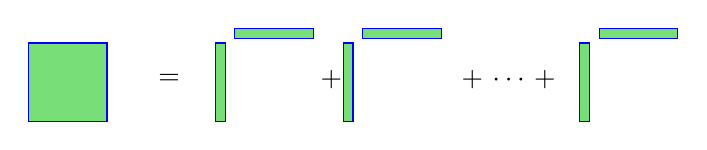
\begin{tikzpicture}[scale=0.25, every node/.style={transform shape}]
\pgfmathsetmacro{\cubex}{4}
\pgfmathsetmacro{\cubey}{4}
\pgfmathsetmacro{\cubez}{4}
\draw[blue,fill=pastelgreen] (0,0,0) -- ++(-\cubex,0,0) -- ++(0,-\cubey,0) -- ++(\cubex,0,0) -- cycle;
%%\draw[blue,fill=pastelgreen] (0,0,0) -- ++(0,0,-\cubez) -- ++(0,-\cubey,0) -- ++(0,0,\cubez) -- cycle;
%%\draw[blue,fill=pastelgreen] (0,0,0) -- ++(-\cubex,0,0) -- ++(0,0,-\cubez) -- ++(\cubex,0,0) -- cycle;

\node[draw=none, text=black, scale=4] at (2,-3,-3) {$=$};
\pgfmathsetmacro{\smallwidth}{0.5}
\draw[blue,fill=pastelgreen] (\cubex+2,0,0) -- ++(-\smallwidth,0,0) -- ++(0,-\cubey,0) -- ++(\smallwidth,0,0) -- cycle;
\draw[blue,fill=pastelgreen] (\cubex+2 +\cubex + 0.5,0.75,0) -- ++(-\cubex,0,0) -- ++(0,-\smallwidth,0) -- ++(\cubex,0,0) -- cycle;
%%\draw[blue,fill=pastelgreen] (\cubex+2,0.5,0) -- ++(-\smallwidth,0,0) -- ++(0,0,-\cubez) -- ++(\smallwidth,0,0) -- cycle;

\node[draw=none, text=black, scale=4] at (2+\cubex+4.25,-3,-3) {$+$};

\draw[blue,fill=pastelgreen] (\cubex+2.5 + \cubex+2,0,0) -- ++(-\smallwidth,0,0) -- ++(0,-\cubey,0) -- ++(\smallwidth,0,0) -- cycle;
\draw[blue,fill=pastelgreen] (\cubex+2.5+\cubex+2 +\cubex + 0.5,0.75,0) -- ++(-\cubex,0,0) -- ++(0,-\smallwidth,0) -- ++(\cubex,0,0) -- cycle;
%%\draw[blue,fill=pastelgreen] (\cubex+2.5+\cubex+2,0.5,0) -- ++(-\smallwidth,0,0) -- ++(0,0,-\cubez) -- ++(\smallwidth,0,0) -- cycle;

\node[draw=none, text=black, scale=4] at (2+\cubex+5 + \cubex+ 4.25, -3,-3) {$+$ $\cdots$ $+$};

\draw[blue,fill=pastelgreen] (12 + \cubex+2.5 + \cubex+2,0,0) -- ++(-\smallwidth,0,0) -- ++(0,-\cubey,0) -- ++(\smallwidth,0,0) -- cycle;
\draw[blue,fill=pastelgreen] (12+\cubex+2.5+\cubex+2 +\cubex + 0.5,0.75,0) -- ++(-\cubex,0,0) -- ++(0,-\smallwidth,0) -- ++(\cubex,0,0) -- cycle;
%%\draw[blue,fill=pastelgreen] (12 + \cubex+2.5+\cubex+2,0.5,0) -- ++(-\smallwidth,0,0) -- ++(0,0,-\cubez) -- ++(\smallwidth,0,0) -- cycle;
\end{tikzpicture}
\end{center}
\end{frame}

\begin{frame}{Popular Tensor Decompositions}{Higher Order Generalization of SVD}
\begin{itemize}
	\item Canonical decomposition (equivalently known as Canonical Polyadic or CANDECOMP or PARAFAC)
	\vfill
	\item Tucker decomposition
	\vfill
	\item Tensor Train decomposition (equivalently known as Matrix Product States)
	\vfill
\end{itemize}
\begin{block}{Tensor Notations}
	\begin{itemize}
		\item \tensor{A} $\in \mathbb{R}^{n_1 \times \ldots \times n_d}$ is a $d$-dimensional tensor
%%		\item $\tensor{A}(i_1,\cdots,i_d)$ represent elements of $\tensor{A}$
		\item Use bold letters to denote tensors
	\end{itemize}
\end{block}
\end{frame}

\begin{frame}{Canonical Representation}
\begin{center}
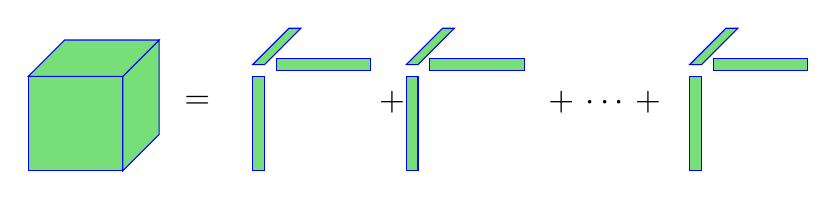
\begin{tikzpicture}[scale=0.3, every node/.style={transform shape}]
\pgfmathsetmacro{\cubex}{4}
\pgfmathsetmacro{\cubey}{4}
\pgfmathsetmacro{\cubez}{4}
\draw[blue,fill=pastelgreen] (0,0,0) -- ++(-\cubex,0,0) -- ++(0,-\cubey,0) -- ++(\cubex,0,0) -- cycle;
\draw[blue,fill=pastelgreen] (0,0,0) -- ++(0,0,-\cubez) -- ++(0,-\cubey,0) -- ++(0,0,\cubez) -- cycle;
\draw[blue,fill=pastelgreen] (0,0,0) -- ++(-\cubex,0,0) -- ++(0,0,-\cubez) -- ++(\cubex,0,0) -- cycle;

\node[draw=none, text=black, scale=4] at (2,-2.25,-3) {$=$};
\pgfmathsetmacro{\smallwidth}{0.5}
\draw[blue,fill=pastelgreen] (\cubex+2,0,0) -- ++(-\smallwidth,0,0) -- ++(0,-\cubey,0) -- ++(\smallwidth,0,0) -- cycle;
\draw[blue,fill=pastelgreen] (\cubex+2 +\cubex + 0.5,0.75,0) -- ++(-\cubex,0,0) -- ++(0,-\smallwidth,0) -- ++(\cubex,0,0) -- cycle;
\draw[blue,fill=pastelgreen] (\cubex+2,0.5,0) -- ++(-\smallwidth,0,0) -- ++(0,0,-\cubez) -- ++(\smallwidth,0,0) -- cycle;

\node[draw=none, text=black, scale=4] at (2+\cubex+4.25,-2.25,-3) {$+$};

\draw[blue,fill=pastelgreen] (\cubex+2.5 + \cubex+2,0,0) -- ++(-\smallwidth,0,0) -- ++(0,-\cubey,0) -- ++(\smallwidth,0,0) -- cycle;
\draw[blue,fill=pastelgreen] (\cubex+2.5+\cubex+2 +\cubex + 0.5,0.75,0) -- ++(-\cubex,0,0) -- ++(0,-\smallwidth,0) -- ++(\cubex,0,0) -- cycle;
\draw[blue,fill=pastelgreen] (\cubex+2.5+\cubex+2,0.5,0) -- ++(-\smallwidth,0,0) -- ++(0,0,-\cubez) -- ++(\smallwidth,0,0) -- cycle;

\node[draw=none, text=black, scale=4] at (2+\cubex+5 + \cubex+ 4.25, -2.25,-3) {$+$ $\cdots$ $+$};

\draw[blue,fill=pastelgreen] (12 + \cubex+2.5 + \cubex+2,0,0) -- ++(-\smallwidth,0,0) -- ++(0,-\cubey,0) -- ++(\smallwidth,0,0) -- cycle;
\draw[blue,fill=pastelgreen] (12+\cubex+2.5+\cubex+2 +\cubex + 0.5,0.75,0) -- ++(-\cubex,0,0) -- ++(0,-\smallwidth,0) -- ++(\cubex,0,0) -- cycle;
\draw[blue,fill=pastelgreen] (12 + \cubex+2.5+\cubex+2,0.5,0) -- ++(-\smallwidth,0,0) -- ++(0,0,-\cubez) -- ++(\smallwidth,0,0) -- cycle;

\end{tikzpicture}
\end{center}

\begin{itemize}
\item $\tensor{A}(i_1,\cdots,i_d) = \sum_{\alpha=1}^{r} U_1(i_1,\alpha) U_2(i_2,\alpha)\cdots U_d(i_d,\alpha)$
%%	\item The minimum value of $r$ is called the canonical rank
\end{itemize}
\medspace
\begin{itemize}
\item ({\color{green}+})  For $n_1=n_2=\cdots n_d=n$, the number of entries = $\mathcal{O}(nrd)$
\item ({\color{red}-}) Determining the minimum value of $r$ is an NP-complete problem
\item ({\color{red}-}) No robust algorithms to compute this representation
\end{itemize}
\end{frame}

\begin{frame}{Tucker Representation}
\begin{center}
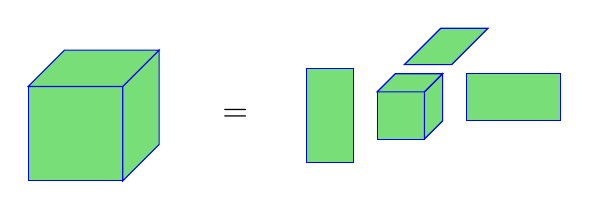
\begin{tikzpicture}[scale=0.3, every node/.style={transform shape}]
\pgfmathsetmacro{\cubex}{4}
\pgfmathsetmacro{\cubey}{4}
\pgfmathsetmacro{\cubez}{4}
\draw[blue,fill=pastelgreen] (-12,1,\cubez-2) -- ++(-\cubex,0,0) -- ++(0,-\cubey,0) -- ++(\cubex,0,0) -- cycle;
\draw[blue,fill=pastelgreen] (-12,1,\cubez-2) -- ++(0,0,-\cubez) -- ++(0,-\cubey,0) -- ++(0,0,\cubez) -- cycle;
\draw[blue,fill=pastelgreen] (-12,1,\cubez-2) -- ++(-\cubex,0,0) -- ++(0,0,-\cubez) -- ++(\cubex,0,0) -- cycle;
\node[draw=none, text=black, scale=4] at (-8,-1,0) {$=$};

\pgfmathsetmacro{\cubex}{2}
\pgfmathsetmacro{\cubey}{2}
\pgfmathsetmacro{\cubez}{2}
\draw[blue,fill=pastelgreen] (0,0,0) -- ++(-\cubex,0,0) -- ++(0,-\cubey,0) -- ++(\cubex,0,0) -- cycle;
\draw[blue,fill=pastelgreen] (0,0,0) -- ++(0,0,-\cubez) -- ++(0,-\cubey,0) -- ++(0,0,\cubez) -- cycle;
\draw[blue,fill=pastelgreen] (0,0,0) -- ++(-\cubex,0,0) -- ++(0,0,-\cubez) -- ++(\cubex,0,0) -- cycle;

\draw[blue,fill=pastelgreen] (-\cubex-1,1,0) -- ++(-\cubex,0,0) -- ++(0,-\cubey-2,0) -- ++(\cubex,0,0) -- cycle;
\draw[blue,fill=pastelgreen] (\cubex+2+1,0,-\cubey) -- ++(-\cubex-2,0,0) -- ++(0,-\cubey,0) -- ++(\cubex+2,0,0) -- cycle;

\draw[blue,fill=pastelgreen] (0,0,-\cubez-1) -- ++(-\cubex,0,0) -- ++(0,0,-\cubez-2) -- ++(\cubex,0,0) -- cycle;
\end{tikzpicture}
\end{center}

\begin{itemize}
\item Represents a tensor with $d$ matrices and a small core tensor
\item $\tensor{A}(i_1,\cdots,i_d) = \sum_{\alpha_1=1}^{r_1}\cdots\sum_{\alpha_d=1}^{r_d} \tensor{g}_{\alpha_1\cdots\alpha_d}U_1(i_1,\alpha_1)$ $\cdots U_d(i_d, \alpha_d)$
\medspace
\end{itemize}
\medspace
\begin{itemize}
\item ({\color{green}+}) SVD based stable algorithms to compute this representation
\item ({\color{red}-})  For $n_1=n_2=\cdots n_d=n$ and $r_1=r_2=\cdots =r_d=r$, the number of entries = $\mathcal{O}(ndr+r^d)$
\end{itemize}	
\end{frame}

%------------------------------------------------
\begin{frame}{Tensor Train Representation: Product of Matrices View}
\begin{itemize}
\item A $d$-dimensional tensor is represented with $2$ matrices and $d$-$2$ $3$-dimensional tensors.
\end{itemize}
\begin{figure}
\begin{center}	
\includegraphics[scale=0.35]{./diagrams/ttentry.eps}
\end{center}
\end{figure}
\noindent An entry of $\tensor{A}$ $\in$ $\mathbb{R}^{n_1 \times \cdots \times n_d}$ is computed by multiplying corresponding matrix (or row/column) of each core.
\end{frame}

\begin{frame}{Tensor Train Representation}

\begin{block}{}
$\tensor{A}$ $\in$ $\mathbb{R}^{n_1 \times \cdots \times n_d}$ is represented with cores $\tensor{G}_k$$\in$ $\mathbb{R}^{r_{k-1}\times n_k\times r_k}$, $k$=$1,2,\cdots d$, $r_0$=$r_d$=$1$ and its elements satisfy the following expression:
{\small\begin{align*}
\tensor{A}(i_1,\cdots ,i_d) 
&= \sum_{\alpha_0 = 1}^{r_0} \cdots \sum_{\alpha_d = 1}^{r_d} \tensor{G}_1(\alpha_0, i_1, \alpha_1) \cdots \tensor{G}_d(\alpha_{d-1}, i_d, \alpha_d)\\
&= \sum_{\alpha_1 = 1}^{r_1} \cdots \sum_{\alpha_{d-1} = 1}^{r_{d-1}} \tensor{G}_1(1, i_1, \alpha_1) \cdots \tensor{G}_d(\alpha_{d-1}, i_d, 1)
\end{align*}}
\begin{center}
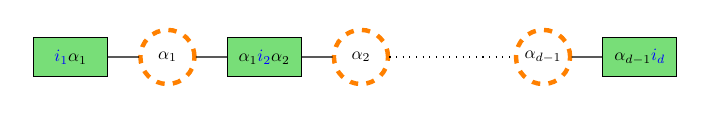
\begin{tikzpicture}[scale=0.625, every node/.style={transform shape}]
\tikzstyle{taskc}=[circle, draw=orange, minimum size=11mm, fill=none, dashed, ultra thick]
\tikzstyle{taskr}=[draw=black, minimum height=8mm, minimum width=15mm, anchor=south west, fill=pastelgreen, text=black]

\node(t1) at (0,0) {};
\node [above right=0cm and 0cm of t1.mid,taskr](T1) {$\textcolor{blue}{i_1}\alpha_1$};
\node [above right=0cm and 0.8cm of T1.south east, taskc](C1) {$\alpha_1$};
\node [above right=0cm and 0.8cm of C1.south east, taskr](T2) {$\alpha_1\textcolor{blue}{i_2}\alpha_2$};
\node [above right=0cm and 0.8cm of T2.south east, taskc](C2) {$\alpha_2$};

\node [above right=0cm and 4.5cm of T2.south east, taskc](Cd) {$\alpha_{d\text{-}1}$};
\node [above right=0cm and 0.8cm of Cd.south east, taskr](Td) {$\alpha_{d\text{-}1}\textcolor{blue}{i_d}$};
\draw (T1.east)--(C1.west);
\draw (C1.east)--(T2.west);
\draw (T2.east)--(C2.west);
\draw [dotted] (C2.east)--(Cd.west);
\draw (Cd.east)--(Td.west);
\path (-0.1, -0.4) -- (2.5, -0.4); 
%%\path (-0.1, -0.8) -- (2.5, -0.8); 
\end{tikzpicture}
\end{center}
\end{block}
\begin{itemize}
\item For $n_1=n_2=\cdots=n_d=n$ and $r_1=r_2=\cdots=r_{d-1}=r$, the number of entries = $\mathcal{O}(ndr^2)$
\end{itemize}
\end{frame}



\begin{frame}{$2\times 2$ Matrix multiplication as a tensor operation}
\begin{align*}
\begin{pmatrix}
C_{11} & C_{12} \\
C_{21} & C_{22}
\end{pmatrix}
&
=
\begin{pmatrix}
A_{11} & A_{12} \\
A_{21} & A_{22}
\end{pmatrix}
\begin{pmatrix}
B_{11} & B_{12} \\
B_{21} & B_{22}
\end{pmatrix}
\end{align*}

We can write this multiplication as a tensor operation,
\begin{align*}
\tensor{T}\times_1 \begin{pmatrix}
A_{11}\\
A_{12}\\
A_{21}\\
A_{22}
\end{pmatrix}
\times_2 \begin{pmatrix}
B_{11}\\
B_{12}\\
B_{21}\\
B_{22}
\end{pmatrix}
&=\begin{pmatrix}
C_{11}\\
C_{12}\\
C_{21}\\
C_{22}
\end{pmatrix}
\end{align*}
\only<1>{
Where \tensor{T} is a $4\times4\times4$ tensor with the following slices:
\begin{align*}\tiny
T_1= \begin{pmatrix}
1&0&0&0\\
0&0&1&0\\
0&0&0&0\\
0&0&0&0
\end{pmatrix}
&\tiny
T_2= \begin{pmatrix}
0&1&0&0\\
0&0&0&1\\
0&0&0&0\\
0&0&0&0
\end{pmatrix}
&\tiny
T_3= \begin{pmatrix}
0&0&0&0\\
0&0&0&0\\
1&0&0&0\\
0&0&1&0
\end{pmatrix}
&\tiny
T_4= \begin{pmatrix}
0&0&0&0\\
0&0&0&0\\
0&1&0&0\\
0&0&0&1
\end{pmatrix}
\end{align*}
}
\only<2>{
	For example,
	\tiny
	
	\begin{align*}
	T_2\times_1 \begin{pmatrix}
	A_{11}\\
	A_{12}\\
	A_{21}\\
	A_{22}
	\end{pmatrix}
	\times_2 \begin{pmatrix}
	B_{11}\\
	B_{12}\\
	B_{21}\\
	B_{22}
	\end{pmatrix}
	&=(
	A_{11}\text{ }
	A_{12}\text{ }
	A_{21}\text{ }
	A_{22})
	\begin{pmatrix}
		0&1&0&0\\
		0&0&0&1\\
		0&0&0&0\\
		0&0&0&0
	\end{pmatrix}
	\begin{pmatrix}
	B_{11}\\
	B_{12}\\
	B_{21}\\
	B_{22}
	\end{pmatrix}
	=A_{11}B_{12} + A_{12}B_{22} =C_{12}
	\end{align*}
}



\end{frame}
\begin{frame}{Matrix multiplication with canonical low rank decomposition}
Canonical low rank decomposition of \tensor{T} can be written as,
\begin{align*}
\tensor{T}&= \sum_{r=1}^{R}u_r \circ v_r \circ w_r
\end{align*}
We can write matrix multiplication as,
{\tiny
\begin{align*}
\tensor{T}\times_1 \begin{pmatrix}
A_{11}\\
A_{12}\\
A_{21}\\
A_{22}
\end{pmatrix}
\times_2 \begin{pmatrix}
B_{11}\\
B_{12}\\
B_{21}\\
B_{22}
\end{pmatrix}
&= \sum_{r=1}^{R}(u_r \circ v_r \circ w_r)
\times_1 \begin{pmatrix}
A_{11}\\
A_{12}\\
A_{21}\\
A_{22}
\end{pmatrix}
\times_2 \begin{pmatrix}
B_{11}\\
B_{12}\\
B_{21}\\
B_{22}
\end{pmatrix}\\
&=\sum_{r=1}^{R}\Big[
\text{($A_{11}$ $A_{12}$ $A_{21}$ $A_{22}$)}u_r
\text{($B_{11}$ $B_{12}$ $B_{21}$ $B_{22}$)}v_r
 \Big]w_r
 =\begin{pmatrix}
 C_{11}\\
 C_{12}\\
 C_{21}\\
 C_{22}
 \end{pmatrix}
\end{align*}
}
\end{frame}
\begin{frame}{Factor matrices and Strassen's algorithm}

\begin{minipage}{0.45\linewidth}
{\small
Factor matrices,
\begin{align*}
u&=\begin{pmatrix}
1& 0& 1& 0& 1& -1& 0&\\
0& 0& 0& 0& 1& 0& 1&\\
0& 1& 0& 0& 0& 1& 0&\\
1& 1& 0& 1& 0& 0& -1&
\end{pmatrix}\\
v&=\begin{pmatrix}
1& 1& 0& -1& 0& 1& 0&\\
0& 0& 1& 0& 0& 1& 0&\\
0& 0& 0& 1& 0& 0& 1&\\
1& 0& -1& 0& 1& 0& 1&
\end{pmatrix}\\
w&=\begin{pmatrix}
1& 0& 0& 1& -1& 0& 1&\\
0& 0& 1& 0& 1& 0& 0&\\
0& 1& 0& 1& 0& 0& 0&\\
1& -1& 1& 0& 0& 1& 0&
\end{pmatrix}
\end{align*}}
\end{minipage}
\begin{minipage}{0.45\linewidth}
{\small Strassen's algorithm,
	\begin{align*}\small
	M_1 &= (A_{11} + A_{22})(B_{11}+B_{22})\\
	M_2 &= (A_{21} + A_{22})B_{11}\\
	M_3 &= A_{11} (B_{12}-B_{22})\\
	M_4 &= A_{22} (B_{21}-B_{11})\\
	M_5 &= (A_{11} +A_{12})B_{22}\\
	M_6 &= (A_{21}-A_{11})(B_{11} +B_{12})\\
	M_7 &= (A_{12}-A_{22})(B_{21} + B_{22}) 
	\end{align*}
	\begin{align*}
	C_{11} &= M_1 + M_4 -M_5 +M_7\\
	C_{12} &= M_3 + M_5\\
	C_{21} &= M_2 + M_4\\
	C_{22} &= M_1 -M_2 + M_3 + M_6
	\end{align*}
}\end{minipage}
\vfill
Factor matrices $u$, $v$, and $w$ construct the algorithm.
\end{frame}
\section{Cost Analysis of Traditional Matrix Multiplication Algorithm}
\begin{frame}
\frametitle{Table of Contents}
\tableofcontents[currentsection]
\end{frame}
\begin{frame}{Communication and computation costs}
Algorithms have two types of costs:
\begin{itemize}
	\item Computation costs (Floating point operations per second)
	\item Communication costs
	\begin{itemize}
		\item Cost to move data between two levels of a memory hierarchy
	\end{itemize}
\end{itemize}

\begin{center}
	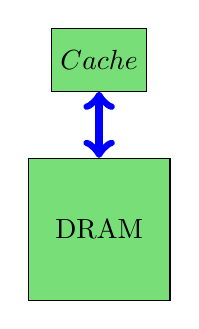
\begin{tikzpicture}[scale=1, every node/.style={transform shape}]
	%%	\tikzstyle{taskr}=[draw=black, minimum height=18mm, minimum width=18mm, anchor=south west, fill=pastelgreen, text=black]
	
	\tikzstyle{taskr}=[draw=black, minimum height=18mm, minimum width=18mm, fill=pastelgreen, text=black]
	
	\tikzstyle{taskrsmall}=[draw=black, minimum height=8mm, minimum width=8mm, fill=pastelgreen, text=black]
	
	%%	\node(t1) at (0,0) {};
	%%	\node [above right=0cm and 0cm of t1.mid,taskr](T1) {};
	\node [taskrsmall] (T1) at (0,0) {$Cache$};
%%	\node [taskrsmall] (T2) at (T1.mid) {};
%%	\node [above] at (T2.mid) {\tiny C(i,j)};
%%	\node[draw=none, text=black, scale=1] at (2.25,0) {$=$};
%%	
%%	\node [right=3cm of T1.mid,taskr, fill=none](T3) {};
%%	\node[taskrow](T4) at (T3.mid) {};
%%	\node [above] at (T4.mid) {\tiny A(i,:)};
	
	\node [below=1.2cm of T1.mid,taskr](T2) {DRAM};
	\draw [<->,blue, line width=0.1cm](T1.south) -- (T2.north);
	\end{tikzpicture}
\end{center}
\end{frame}
\begin{frame}{Communication costs}
\begin{itemize}
	\item Amount of data -- bandwidth cost
	\item number of messages -- latency cost
\end{itemize}
\begin{block}{Annual rate of improvement}
	\begin{center}
\begin{tabular}{|c|c|c|}
	\hline
	Computations & Bandwidth & Latency\\ \hline
	59\% & 23\% & 5\% \\ \hline
\end{tabular}
	\end{center}
\end{block}
\end{frame}
\begin{frame}[fragile]{Analysis of traditional matrix multiplication algorithm}
	\begin{verbatim}
//implements C=C+AB
for i=1 to n
  for j=1 to n
    for k=1 to n
      C(i,j) = C(i,j) + A(i,k) * B(k,j);
\end{verbatim}
%%\only<2>{\begin{verbatim}
%%	//implements C =C+AB
%%	for i=1 to n
%%	// read row i of A into fast memory  (total n read) 
%%	for j=1 to n
%%	// read row i of C into fast memory (total n read)
%%	// read column j of B into fast memory (total n read)
%%	for k=1 to n
%%	  C(i,j) = C(i,j) + A(i,k) * B(k,j);
%%	  // write row i of C back to slow memory (total n read)
%%	\end{verbatim}
%%$n^2 + 3n^2$ reads/writes combined dominates $2n^3$ computations}
\end{frame}

\begin{frame}[fragile]{Analysis of traditional matrix multiplication algorithm}
\begin{verbatim}
	//implements C=C+AB
	for i=1 to n
	// read row i of A into fast memory  (total n*n reads) 
  	  for j=1 to n
	    // read row i of C into fast memory (total n*n reads)
	    // read column j of B into fast memory (total n*n*n reads)
	    for k=1 to n
	      C(i,j) = C(i,j) + A(i,k) * B(k,j);
	      // write row i of C back to slow memory (total n*n writes)
	\end{verbatim}
	\medskip
$n^3 + 3n^2$ reads/writes combined dominates $2n^3$ computations.
\end{frame}

\begin{frame}[fragile]{Tiled matrix multiplication}
\begin{verbatim}
//Consider, A, B, C to be n/b X n/b matrices of b X b subblocks
//Asumme 3 bXb blocks fit in fast memory
for i=1 to n/b
  for j=1 to n/b
    // read block C(i,j) into fast memory 
    // (total b*b*n/b*n/b = n*n reads)
	for k=1 to n/b
      // read block A(i,k) into fast memory 
      // (total b*b*n/b*n/b*n/b = n*n*n/b reads)
      // read block B(k,j) into fast memory 
      // (total b*b*n/b*n/b*n/b = n*n*n/b reads)
	    C(i,j) = C(i,j) + A(i,k) * B(k,j); //Matrix multiplication in blocks
	    // write block C(i,j) into fast memory 
	    // (total b*b*n/b*n/b = n*n writes)
\end{verbatim}
	\medskip
$\frac{2n^3}{b} + 2n^2$ reads/writes $<<$ $2n^3$ computations.
\end{frame}

\begin{frame}{Amount of volume in matrix multiplication }
\begin{itemize}
	\item Make b as large as possible, 3$b^2 \le M$
	\item Number of reads/writes $\ge 3^\frac{1}{2}n^3/M^\frac{1}{2} + 2n^2$
\end{itemize}
\vfill
\begin{block}{Amount of data lower bound}
For any $3$ nesting loop,
\begin{itemize}
	\item Amount of data = $\Omega(\frac{\#computations}{M^\frac{1}{2}})$
\end{itemize}
\end{block}
\end{frame}

%%\begin{frame}{Extension of bounds to parallel architectures}
%%content...
%%\end{frame}



\section{Tensor Contractions}
\begin{frame}
\frametitle{Table of Contents}
\tableofcontents[currentsection]
\end{frame}

\begin{frame}{Tensor contractions (generalization of matrix multiplication)}
 It contracts the $i$-th dimension of tensor $\tensor{A}$ $\in$ $\mathbb{R}^{n_1 \times n_2 \times \cdots \times n_{d_1}}$ with the $j$-th dimension of tensor $\tensor{B}$ $\in$ $\mathbb{R}^{m_1 \times m_2 \times \cdots \times m_{d_2}}$, where $n_i=m_j$. It is denoted as $\tensor{A}\times_{n_i}\tensor{B}$.
 
%%For $d_1=3$, $d_2=2$, $n_1=n_2=n_3=m_1=m_2=n$, $i=3$, and $j=1$. We assume that the output tensor is $\tensor{G}$ and its all elements are initialized to zero. We can compute $\tensor{G}$ with the following algorithm:
\begin{itemize}
	\item $d_1=3$, $d_2=2$, $n_1=n_2=n_3=m_1=m_2=n$, $i=3$, and $j=1$
	\item Output tensor is $\tensor{G}$ and its all elements are initialized to zero
\end{itemize}
%%\end{frame}
%%\begin{frame}{Tensor contractions}
	\begin{algorithmic}
	\FOR{$i_1=1:n$}
	\FOR{$i_2=1:n$}
	\FOR{$i_3=1:n$}
	\FOR{$j_2=1:n$} 
	\STATE {$\tensor{G}(i_1,i_2,j_2) = \tensor{G}(i_1,i_2,j_2) + \tensor{A}(i_1,i_2,i_3)*\tensor{B}(i_3,j_2)$} 
	\ENDFOR
	\ENDFOR
	\ENDFOR
	\ENDFOR
\end{algorithmic}
\end{frame}
\begin{frame}{Tensor contraction example}
	\begin{algorithmic}
	\FOR{$i_1=1:n$}
	\FOR{$i_2=1:n$}
	\FOR{$i_3=1:n$}
	\FOR{$j_2=1:n$} 
	\STATE {$\tensor{G}(i_1,i_2,j_2) = \tensor{G}(i_1,i_2,j_2) + \tensor{A}(i_1,i_2,i_3)*\tensor{B}(i_3,j_2)$} 
	\ENDFOR
	\ENDFOR
	\ENDFOR
	\ENDFOR
\end{algorithmic}
\begin{itemize}
	\item Total $\mathcal{O}(n^{4})$ operations
	\item Applying Strassen's algorithm for each $i_1$, total $\mathcal{O}(n^{3.81})$ operations 
\end{itemize}
\end{frame}

\begin{frame}{Tensor contractions with Strassen's concept}
\begin{itemize}
	\item Expressing this computation as canonical low rank decomposition of $8\times8\times4$ tensor can further reduce the number of operations
\end{itemize}
\begin{align*}
\tensor{T}\times_1 \begin{pmatrix}
\tensor{A}_{111}\\
\tensor{A}_{112}\\
\tensor{A}_{121}\\
\tensor{A}_{122}\\
\tensor{A}_{211}\\
\tensor{A}_{212}\\
\tensor{A}_{221}\\
\tensor{A}_{222}
\end{pmatrix}
\times_2 \begin{pmatrix}
B_{11}\\
B_{12}\\
B_{21}\\
B_{22}
\end{pmatrix}
&=\begin{pmatrix}
\tensor{G}_{111}\\
\tensor{G}_{112}\\
\tensor{G}_{121}\\
\tensor{G}_{122}\\
\tensor{G}_{211}\\
\tensor{G}_{212}\\
\tensor{G}_{221}\\
\tensor{G}_{222}
\end{pmatrix}
\end{align*}
\end{frame}

\begin{frame}{Multiple tensor contractions($\tensor{A} \times_1 M_1 \times_2 M_2$)}
%%	This computation multiplies a tensor $\tensor{A}$ $\in$ $\mathbb{R}^{n_1 \times n_2 \times \cdots \times n_d}$ with matrices $M_1\in \mathbb{R}^{n_1 \times m_1}$, $\cdots$, $M_k\in \mathbb{R}^{n_k \times m_k}$ in $1$st,$\cdots$, $k$th modes respectively ($k\le d$), and represented as $\tensor{A}\times_1 M_1\times_2 \cdots \times_k M_k$. This is used in 
%%	HOSVD, a tucker decomposition algorithm, to generate a core tensor from the original tensor and factor matrices. One approach to perform this computation is to apply tensor contraction many times. Another approach is to express the computation with $d+k$ \textbf{for} loops and perform arithmetic operations in the innermost loop. Let $\tensor{G}$ be the output tensor and its all elements are initialized to zero. For $d=k=2$, both approaches can be expressed with the following algorithms.
%%	\medskip
	\begin{minipage}{0.45\textwidth}{\footnotesize
			\noindent\underline{Applying tensor contraction twice}\\
			\begin{itemize}
				\item[$*$] \tensor{Tmp} is an intermediate variable
			\end{itemize}	 			
			\begin{algorithmic}
				\FOR{$i_1=1:n_1$}
				\FOR{$i_2=1:n_2$}
				\FOR{$i_{m1}=1:m_1$}
				\STATE {$\tensor{Tmp}(i_{m1},i_2) += \tensor{A}(i_1,i_2)*M_1(i_1,i_{m1})$} 
				\ENDFOR
				\ENDFOR
				\ENDFOR
			\end{algorithmic}
			
			\begin{algorithmic}
				\FOR{$i_2=1:n_2$}
				\FOR{$i_{m1}=1:m_1$}
				\FOR{$i_{m2}=1:m_2$} 
				\STATE {$\tensor{G}(i_{m1},i_{m2})+= \tensor{Tmp}(i_{m1},i_2)*M_2(i_2,i_{m2})$} 
				\ENDFOR
				\ENDFOR
				\ENDFOR
		\end{algorithmic}}
	\end{minipage}
	\hfill
	\begin{minipage}[!h]{0.45\textwidth}{\footnotesize
			\noindent\underline{Computations with $d+k$ \textbf{for} loops}
			\begin{algorithmic}
				\FOR{$i_1=1:n_1$}
				\FOR{$i_2=1:n_2$}
				\FOR{$i_{m1}=1:m_1$}
				\FOR{$i_{m2}=1:m_2$} 
				\STATE {$\tensor{G}(i_{m1},i_{m2}) += \tensor{A}(i_1,i_2)*M_1(i_1,i_{m1}) *M_2(i_2,i_{m2})$} 
				\ENDFOR
				\ENDFOR
				\ENDFOR
				\ENDFOR
		\end{algorithmic}}
		\vfill
	\end{minipage}
	
%%	\noindent Both approaches perform different amount of operations and data transfers between levels of a memory hierarchy. There are multiple ways to performs this computation. I plan to obtain the lower bounds, determining the minimum amount of operations and data transfers between different levels of memory or among parallel processors over a network required to perform Multi-TTM computations, and design algorithms which achieve both bounds simultaneously if possible.
\end{frame}

\begin{frame}{Multiple tensor contractions($\tensor{A} \times_1 M_1 \times_2 M_2$)}
\begin{itemize}
	\item Both approaches perform different amount of operations and communications
	\vfill
	\item Multiple ways to perform this computation
	\vfill
	\item Known as Multi-Tensor Times Matrix (Multi-TTM) computation
	\vfill
\end{itemize}
\end{frame}
\section{Conclusion}
\begin{frame}
\frametitle{Table of Contents}
\tableofcontents[currentsection]
\end{frame}


\begin{frame}{Conclusion \& Ongoing Work}
\begin{block}{Conclusion}
\begin{itemize}
	\item Overview of different ways to perform matrix multiplication
	\item Overview of tensors and their low rank decompositions
	\item Connection between Strassen's algorithm and canonical low rank decomposition
	\item Extension of Strassen's concept to tensor contractions
%%	\item Proposed parallel algorithms to compute tensor train decomposition and approximation of a tensor
%%	\item LSB approach achieves similar compression to the sequential algorithm
%%	\item Accuracies of all approaches are within prescribed limit
\end{itemize}

\end{block}
\begin{block}{Ongoing Work}
\begin{itemize}
	\item Lower bounds on the number of operations for tensor contractions
	\item Communication lower bounds for tensor contractions and Multi-TTM operations
\end{itemize}
\end{block}
\end{frame}


%%\begin{frame}
%%\frametitle{References}
%%\footnotesize{
%%	\begin{thebibliography}{99} % Beamer does not support BibTeX so references must be inserted manually as below
%%		\bibitem[OSELEDETS, 2011]{p1} I. V. Oseledets
%%		\newblock Tensor-Train Decomposition
%%		\newblock \emph{SIAM J. Sci. Comput.}, 33(5), 2295–2317.
%%		
%%		\bibitem[Grigori, 2021]{p2} L. Grigori, S. Kumar
%%		\newblock Parallel Tensor Train through Hierarchical Decomposition
%%		\newblock HAL Tech Report, \emph{https://hal.inria.fr/hal-03081555}.
%%		
%%	\end{thebibliography}
%%}
%%\end{frame}

%------------------------------------------------

\begin{frame}
\Huge{\centerline{Thank You!}}
\end{frame}




%%
%%%------------------------------------------------
%%\section{First Section} % Sections can be created in order to organize your presentation into discrete blocks, all sections and subsections are automatically printed in the table of contents as an overview of the talk
%%%------------------------------------------------
%%
%%\subsection{Subsection Example} % A subsection can be created just before a set of slides with a common theme to further break down your presentation into chunks
%%
%%\begin{frame}
%%\frametitle{Paragraphs of Text}
%%Sed iaculis dapibus gravida. Morbi sed tortor erat, nec interdum arcu. Sed id lorem lectus. Quisque viverra augue id sem ornare non aliquam nibh tristique. Aenean in ligula nisl. Nulla sed tellus ipsum. Donec vestibulum ligula non lorem vulputate fermentum accumsan neque mollis.\\~\\
%%
%%Sed diam enim, sagittis nec condimentum sit amet, ullamcorper sit amet libero. Aliquam vel dui orci, a porta odio. Nullam id suscipit ipsum. Aenean lobortis commodo sem, ut commodo leo gravida vitae. Pellentesque vehicula ante iaculis arcu pretium rutrum eget sit amet purus. Integer ornare nulla quis neque ultrices lobortis. Vestibulum ultrices tincidunt libero, quis commodo erat ullamcorper id.
%%\end{frame}
%%
%%%------------------------------------------------
%%
%%\begin{frame}
%%\frametitle{Bullet Points}
%%\begin{itemize}
%%\item Lorem ipsum dolor sit amet, consectetur adipiscing elit
%%\item Aliquam blandit faucibus nisi, sit amet dapibus enim tempus eu
%%\item Nulla commodo, erat quis gravida posuere, elit lacus lobortis est, quis porttitor odio mauris at libero
%%\item Nam cursus est eget velit posuere pellentesque
%%\item Vestibulum faucibus velit a augue condimentum quis convallis nulla gravida
%%\end{itemize}
%%\end{frame}
%%
%%%------------------------------------------------
%%
%%\begin{frame}
%%\frametitle{Blocks of Highlighted Text}
%%\begin{block}{Block 1}
%%Lorem ipsum dolor sit amet, consectetur adipiscing elit. Integer lectus nisl, ultricies in feugiat rutrum, porttitor sit amet augue. Aliquam ut tortor mauris. Sed volutpat ante purus, quis accumsan dolor.
%%\end{block}
%%
%%\begin{block}{Block 2}
%%Pellentesque sed tellus purus. Class aptent taciti sociosqu ad litora torquent per conubia nostra, per inceptos himenaeos. Vestibulum quis magna at risus dictum tempor eu vitae velit.
%%\end{block}
%%
%%\begin{block}{Block 3}
%%Suspendisse tincidunt sagittis gravida. Curabitur condimentum, enim sed venenatis rutrum, ipsum neque consectetur orci, sed blandit justo nisi ac lacus.
%%\end{block}
%%\end{frame}
%%
%%%------------------------------------------------
%%
%%\begin{frame}
%%\frametitle{Multiple Columns}
%%\begin{columns}[c] % The "c" option specifies centered vertical alignment while the "t" option is used for top vertical alignment
%%
%%\column{.45\textwidth} % Left column and width
%%\textbf{Heading}
%%\begin{enumerate}
%%\item Statement
%%\item Explanation
%%\item Example
%%\end{enumerate}
%%
%%\column{.5\textwidth} % Right column and width
%%Lorem ipsum dolor sit amet, consectetur adipiscing elit. Integer lectus nisl, ultricies in feugiat rutrum, porttitor sit amet augue. Aliquam ut tortor mauris. Sed volutpat ante purus, quis accumsan dolor.
%%
%%\end{columns}
%%\end{frame}
%%
%%%------------------------------------------------
%%\section{Second Section}
%%%------------------------------------------------
%%
%%\begin{frame}
%%\frametitle{Table}
%%\begin{table}
%%\begin{tabular}{l l l}
%%\toprule
%%\textbf{Treatments} & \textbf{Response 1} & \textbf{Response 2}\\
%%\midrule
%%Treatment 1 & 0.0003262 & 0.562 \\
%%Treatment 2 & 0.0015681 & 0.910 \\
%%Treatment 3 & 0.0009271 & 0.296 \\
%%\bottomrule
%%\end{tabular}
%%\caption{Table caption}
%%\end{table}
%%\end{frame}
%%
%%%------------------------------------------------
%%
%%\begin{frame}
%%\frametitle{Theorem}
%%\begin{theorem}[Mass--energy equivalence]
%%$E = mc^2$
%%\end{theorem}
%%\end{frame}
%%
%%%------------------------------------------------
%%
%%\begin{frame}[fragile] % Need to use the fragile option when verbatim is used in the slide
%%\frametitle{Verbatim}
%%\begin{example}[Theorem Slide Code]
%%\begin{verbatim}
%%\begin{frame}
%%\frametitle{Theorem}
%%\begin{theorem}[Mass--energy equivalence]
%%$E = mc^2$
%%\end{theorem}
%%\end{frame}\end{verbatim}
%%\end{example}
%%\end{frame}
%%
%%%------------------------------------------------
%%
%%\begin{frame}
%%\frametitle{Figure}
%%Uncomment the code on this slide to include your own image from the same directory as the template .TeX file.
%%%\begin{figure}
%%%\includegraphics[width=0.8\linewidth]{test}
%%%\end{figure}
%%\end{frame}
%%
%%%------------------------------------------------
%%
%%\begin{frame}[fragile] % Need to use the fragile option when verbatim is used in the slide
%%\frametitle{Citation}
%%An example of the \verb|\cite| command to cite within the presentation:\\~
%%
%%This statement requires citation \cite{p1}.
%%\end{frame}
%%
%%%------------------------------------------------
%%
%%\begin{frame}
%%\frametitle{References}
%%\footnotesize{
%%\begin{thebibliography}{99} % Beamer does not support BibTeX so references must be inserted manually as below
%%\bibitem[Smith, 2012]{p1} John Smith (2012)
%%\newblock Title of the publication
%%\newblock \emph{Journal Name} 12(3), 45 -- 678.
%%\end{thebibliography}
%%}
%%\end{frame}
%%
%%%------------------------------------------------
%%
%%\begin{frame}
%%\Huge{\centerline{The End}}
%%\end{frame}

%----------------------------------------------------------------------------------------

\end{document} 